\documentclass[11pt]{article}
\textheight 9in
\textwidth 6.5in
\oddsidemargin 0in
\topmargin 0in
\headheight 1in
\headsep 0in
\usepackage{color}
\usepackage{lastpage}
\usepackage{graphicx}
\usepackage{fancyhdr}
\pagestyle{fancy}
\cfoot{}
\rhead{\thepage\ of \pageref{LastPage}}
% \renewcommand{\headrulewidth}{0pt}
\usepackage[top = 4em, headsep=.2in]{geometry}
\usepackage{textcomp}
\usepackage{enumitem}

\begin{document}

\noindent{{\textbf{\large Spring 2020  \hfill Stat 305 (Section 4)
\hfill %Page \thepage   { of }  \pageref{lastpage}
Quiz 2}}

\vspace{2em}

\noindent\framebox(200, 50){\vspace{3em}\hspace{2em}\bf Name: \hspace{6cm}}

\bigskip

\noindent\emph{Total points for the exam is 50. Points for
individual questions are given at the beginning of each problem.
Show all your calculations clearly. Put final answers in the box at
the right (except for the diagrams!).}


\bigskip


\noindent {\bf 1.}\hfill[6+6+6+2+4+4+2=30 points] \\

\noindent The data used in creating the attached JMP output (Page 5) appear in
the text \emph{Quality Control and Industrial Statistics} by Duncan (and were
from a paper of L. E. Simon). The data were collected in a study of the
effectiveness of armor plate. Armor-piercing bullets were fired at an angle of 40\textdegree{} against armor plate of thickness $x_1$ (in $10^{-3}$ in.) and Brinell hardnessnumber $x_2$, and the resulting so-called ballistic limit, $y$ (in ft/sec), was measured.

\begin{enumerate}[label = (\alph*)]
	\item What were the two least square equations fit to the data ?

\hfill \fbox{ \textcolor[rgb]{1.00,1.00,1.00}{$\bigcap$} \hskip
-0.4cm Equation 1: $\;\hat y =$ \hspace{10cm}}

\hfill \fbox{ \textcolor[rgb]{1.00,1.00,1.00}{$\bigcap$} \hskip
-0.4cm Equation 2: $\; \hat y =$ \hspace{10cm}}


%\vskip 1cm

\item What fraction of the raw variability in the \emph{ballistic
	limit} is
accounted for by the two equations?

\hfill \fbox{ \textcolor[rgb]{1.00,1.00,1.00}{$\bigcap$} \hskip
-0.4cm For equation 1:\hspace{3cm}}

\hfill \fbox{ \textcolor[rgb]{1.00,1.00,1.00}{$\bigcap$} \hskip
-0.4cm For equation 2:\hspace{3cm}}

\vskip 1cm

\item What is the sample correlation between $y$ and $\hat{y}$ by the two
	equations? (Give a number.)

\hfill \fbox{ \textcolor[rgb]{1.00,1.00,1.00}{$\bigcap$} \hskip
-0.4cm For equation 1:\hspace{3cm}}

\hfill \fbox{ \textcolor[rgb]{1.00,1.00,1.00}{$\bigcap$} \hskip
-0.4cm For equation 2:\hspace{3cm}}

\vskip 1cm






\item What is the sample correlation between \emph{ballistic limit} ($y$)
	and \emph{thinkness of the armor plate} ($x_1$)? (Give a number, be
careful about the sign.)

\hfill \fbox{ \textcolor[rgb]{1.00,1.00,1.00}{$\bigcap$} \hskip
-0.4cm $r =$ \hspace{3cm}}

\vskip 1cm
\clearpage
\item Using the {\bf first equation}, what \emph{ballistic limit} would you
	predict when \emph{thinkness of the armor plate} is $251 \times
	10^{-3}$ in. ? Would you be willing to
predict \emph{strength of wood beams} when \emph{moisture content}
is $100 \times 10^{-3}$ in. ? Why or why not?
\vskip 1cm
\hfill \fbox{ \textcolor[rgb]{1.00,1.00,1.00}{$\bigcap$} \hskip
-0.4cm predicted $y =$ \hspace{3cm}}

\vskip 1cm

\hfill \fbox{ \textcolor[rgb]{1.00,1.00,1.00}{$\bigcap$} \hskip
-0.4cm Yes/No ? Why:  \hspace{12cm}}

\vskip 0.5cm



\item Using the {\bf second equation}, find the values of the
	\underline{residuals} for the
	first 2 data points (the first two data points are the
	two observations in the the first row of the
	data table).

\vskip 1cm

\hfill \fbox{ \textcolor[rgb]{1.00,1.00,1.00}{$\bigcap$} \hskip
-0.4cm residual for first data point $ =$ \hspace{3cm}}

\vskip 1cm


\hfill \fbox{ \textcolor[rgb]{1.00,1.00,1.00}{$\bigcap$} \hskip
-0.4cm residual for second data point $ =$ \hspace{3cm}}


\item Using the {\bf second equation}, about what {\bf change} in average
	\emph{ballistic limit} seems to accompany a 2-unit increase in both $x_1$
	and $x_2$? (For $x_1$, one unit is $10^{-3}$ in.)

	\hfill \fbox{ \textcolor[rgb]{1.00,1.00,1.00}{$\bigcap$} \hskip
-0.4cm change in $y =$ \hspace{3cm}}

\vskip 2cm

\end{enumerate}


\noindent {\bf 2.}\hfill[4+4+6=14 points] \\

  Consider a discrete random variable $X$ with the probability mass
function as specified below. The constant $c$ is to be determined.\\

\begin{tabular}{|r|c|c|c|c|c|}
  \hline
  % after \\: \hline or \cline{col1-col2} \cline{col3-col4} ...
  $x$ & $-2$ & $-1$ & $0$ & $1$ & $2$ \\
  \hline
  $f(x)$ & 0.1 & 0.2 & $c$ & 0.2 & 0.3 \\
  \hline
\end{tabular}

\begin{enumerate}[label = (\alph*)]

	\item Determine $c$ and make a probability histogram (barplot) for
		$X$.

\vskip 0.5cm

 \hfill \fbox{ \textcolor[rgb]{1.00,1.00,1.00}{$\bigcap$}
\hskip -0.4cm $c=$ \hspace{3cm}}

\vskip 5cm

\item Find $P(|X| < 2)$ and $P(|X - 1| > 1 )$.



 \hfill \fbox{ \textcolor[rgb]{1.00,1.00,1.00}{$\bigcap$}
 \hskip -0.4cm $P(|X| < 2) = $ \hspace{3cm}}

\vskip 2cm

 \hfill \fbox{ \textcolor[rgb]{1.00,1.00,1.00}{$\bigcap$}
 \hskip -0.4cm $P(|X - 1| > 1) = $ \hspace{3cm}}


\vskip 3cm

\item Find the mean and standard deviation of $X$.

\vskip 1.5cm

 \hfill \fbox{ \textcolor[rgb]{1.00,1.00,1.00}{$\bigcap$}
\hskip -0.4cm $\mu=$ \hspace{3cm}}

\vskip 1cm

 \hfill \fbox{ \textcolor[rgb]{1.00,1.00,1.00}{$\bigcap$}
\hskip -0.4cm $\sigma=$ \hspace{3cm}}

\vskip 0.5cm

\end{enumerate}

\noindent {\bf 3.}\hfill[6 points] \\


  Suppose that 15\% of all daily oxygen purities delivered by an air-products
  supplier are below 99.5\% purity and that it is plausible to think of
  daily purities as independent random variables. Evaluate the probability
  that in the next five-day workweek, 1 or less delivered purities will fall
  below 99.5\%.



\vskip 0.5cm





 \hfill \fbox{ \textcolor[rgb]{1.00,1.00,1.00}{$\bigcap$}
\hskip -0.4cm probability $=$ \hspace{3cm}}




\clearpage
\hspace{0pt}
\vfill

\centering
This page is intended to be blank.

\vfill

\hspace{0pt}
\clearpage

\section*{Data Table}

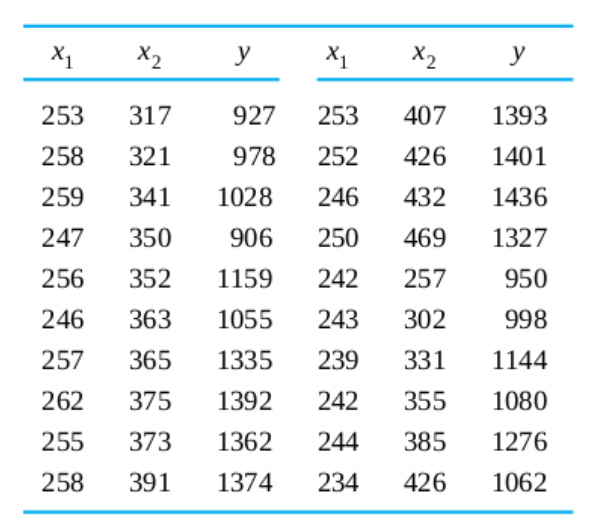
\includegraphics[width = 0.4\textwidth]{./q2data.PNG}

\section*{JMP Output}

\subsection*{Fit 1}

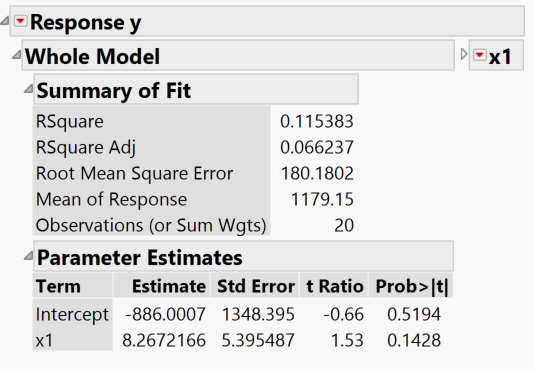
\includegraphics[width = 0.6\textwidth]{./q2x1.PNG}

\subsection*{Fit 2}

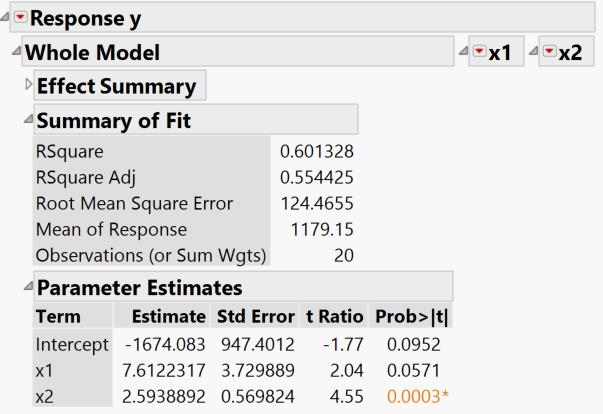
\includegraphics[width =0.6\textwidth]{./q2x1x2.PNG}
%
\label{lastpage}


\end{document}
